\chapter{Editor umožňujúci konkurentné úpravy jedného dokumentu}

\label{kap:zdialtelnost} % id kapitoly pre prikaz ref

Myšlienka kolaboratývneho editora bola prvýkrát zaznamenaná už v roku 1968 Douglas Engelbart-om. 
Avšak do popularity sa dostala až nedávno, približne 20 rokov od prvého záznamu.
Kolaboratívny editor umožnuje viacerým užívaťeľom upravovať jeden dokument.
Tieto editory sa rozďeľujú na dve kategórie
\begin{itemize}
  \item Real time - zmeny dokumentu sa okamžite zobrazia všetkým používateľom
  \item Non-real-time - zmeny dokumentu sa nedejú okamžite (podobne ako pri verzionovacých
  systémoch ako Git, Mercurial)
\end{itemize}
My sa v práci zameriavame real time editormi, kde je treba riešiť synchronizáciu editorových
inštancii používateľov a riešenie možných konfliktov.

\section{Real time kolaboratívnt editor}
Problematika real time kolaboratívnych editorov sa dá rozdeliť do samostatných zmysluplných 
podkapitol
\begin{itemize}
\item  technické výzvy
\item  algoritmy riešiace konkurentné modifikácie jedného zdroja
\end{itemize}

\subsection{Technické výzvy}
Technické vźyvy pramenia z asynchrónnej komunikácie po sieti. Teoreticky, keby táto 
komnikácia bola instantná, tak vytvorenie takéhoto editora, by nebolo priveľmi odlišné od
editora pre jedného používateľa. Algoritmus, rišiaci takýto problém by mohol fungovať na 
základe \textit{upravovacieho zámku}. Fungoval by celkom jednoducho:
\begin{enumerate}
  \item Požiadanie servera o \textit{upravovacý zámok}
  \item Počkanie na schválenie zo servera, že sme na rade s úpravou
  \item Úprava dokumentu
  \item Vzdanie sa \textit{upravovacieho zámku}
\end{enumerate}
Avšak rýchlosť komunikácie je obmedzená latenciou siete. To vytvára základnú dilemu: 
užívatelia potrebujú okamžite vlastné úpravy, ktoré sú do dokumentu zapracované,
ale ak sú začlenené okamžite, potom kvôli latencii komunikácie musia byť ich
úpravy nevyhnutne vložené do rôznych verzií dokumentu.

Problém súbežnej modifikácie jedného textového poľa je, že jednoduché textové operácie ako
pridaj písmeno a zmaž písmneo, nie sú komutatívne \ref{obr:nekomutativita} a ani 
idempotentné \ref{obr:neidempotentnost}. Keďže používatelia
modifikujú dokument cez sieť, nemáme zaručené v akom poradí sa modifikácie uskutočnia. 
\cite {medium_crdt}
Ilustrujme tieto problémy na príklade:

\begin{figure}[h]
\centerline{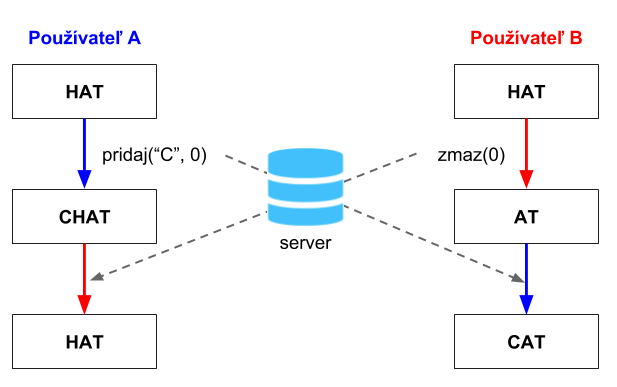
\includegraphics[width=0.6\textwidth]{images/nekomutativne_operacie}}
%popis obrazku
\caption[Nekomutativita textových operácii]{Nekomutativita textových operácii}
%id obrazku, pomocou ktoreho sa budeme na obrazok odvolavat
\label{obr:nekomutativita}
\end{figure}

\begin{figure}[h]
\centerline{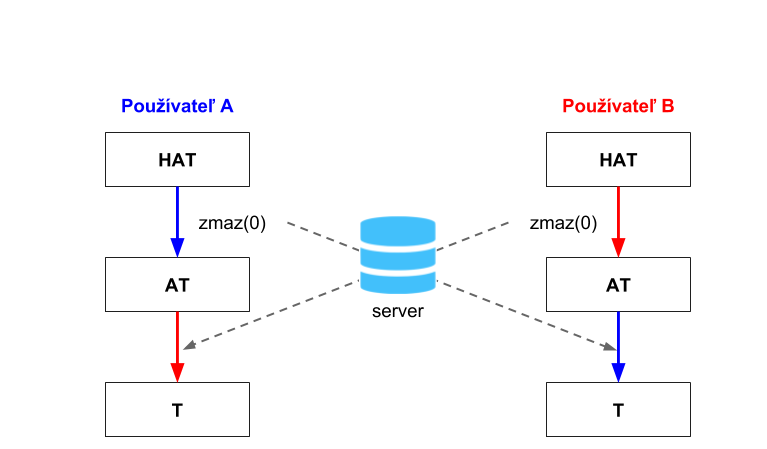
\includegraphics[width=0.6\textwidth]{images/neidempotentne_operacie}}
%popis obrazku
\caption[Neidempotentnosť textových operácii]{Neidempotentnosť textových operácii}
%id obrazku, pomocou ktoreho sa budeme na obrazok odvolavat
\label{obr:neidempotentnost}
\end{figure}

Výzvou v spolupráci v reálnom čase je teda presne zistiť, ako možno aplikovať úpravy
od vzdialených používateľov, ktoré boli pôvodne vytvorené vo verziách dokumentu, ktor
nikdy neexistovali na mieste a ktoré môžu byť v rozpore s vlastnými 
miestnymi úpravami používateľa.

Najsofistikovanejšie riešenia vyriešia tento problém spôsobom, ktorý nevyžaduje server,
nepoužíva uzamknutie (všetci používatelia môžu voľne upravovať všetky časti dokumentu súčasne) 
a podporuje ľubovoľný počet používateľov (obmedzený iba zdrojmi počítačov). 
UNA a SubEthaEdit sú príklady dvoch programov, ktoré využívajú tento prístup.
Tieto programy sú však dostupné iba pre operačných systémoch macOS a využívajú technológie,
ako napríklad \cite{bonjour},ktoré sú špecifické pre tento OS.

Zatiaľ čo tieto sofistikované prístupy umožňujú najlepšiu používateľskú skúsenosť,
v klientskom serveri môže byť vytvorený aj základný editor pre spoluprácu. Pri scenári
klient-server je pri otvorení dokumentu priradená jedna z inštancií editora úloha servera
spolupráce. Tento server zaisťuje, že ostatné editory sú synchronizované určovaním
latencie siete a fungovaním ako server synchronizácie času. Server obdrží upozornenia
na časové označenie zmien vykonaných v dokumente inými používateľmi. 
Určuje, ako majú tieto zmeny ovplyvňovať svoju lokálnu kópiu, a vysiela jej zmeny do
fondu spolupráce. V niektorých modeloch sa zmeny na klienta neodzrkadľujú dovtedy,
kým sa zo servera nevráti oficiálna odpoveď, a to aj vtedy, ak boli tieto zmeny vykonané lokálne.
Príkladom takéhoto editora je napríklad Gobby.

My sme sa v práci rozhodli použiť klient-server model, pričom za synchronizáciu klientov
je zodpovedný výhradne server. Podobný prístup používa napr. spoločnost Google v produktoch
ako Google dokumenty a tabuľky.

\subsection{Algoritmy riešiace konkurentné modifikácie}
Na riešenie synchronizácie klientov existujú dva dobre preskúmané typy algoritmov.
\begin{enumerate}
  \item OT - Prevádzková transformácia (Operational transformation)
  \item CRDT - Bezkonfliktné idempotentné dátové typy (Conflict-free replicated data type)
\end{enumerate}
V práci použijeme CRDT, pretože OT je predchodca CRDT a v praxi často nefunguje tak dobre,
ako to autori zamýšľali. Taktiež použitie OT je komplikované a neškálovateľné \cite{ot_nonscalable}.

\begin{flushleft}\textbf {CRDT \cite{crdt_wiki}}\end{flushleft}

V distribuovanom výpočte je konfliktný replikovaný dátový typ (CRDT) dátová štruktúra,
ktorá môže byť replikovaná vo viacerých počítačoch v sieti, pričom repliky je možné
aktualizovať nezávisle a súbežne bez koordinácie medzi replikami a kde je vždy
matematicky možné vyriešiť nezrovnalosti, ktoré by mohli vyplynúť.

Koncept CRDT bol formálne definovaný v roku 2011 osobami
Marc Shapiro, Nuno Preguiça, Carlos Baquero a Marek Zawirski \cite{crdt_definition}.

CRDT fungujú tak, že každý znak v dokumente sa prerobí do objektu so špecifickými vlastnosťami:
\begin{enumerate}
\label{def_pozicie}
  \item znak, ktoré objekt predstavuje
  \item relatívna pozícia tohto znaku
  \item množina pozícíi musí tvoriť úplné usporiadanie
  \item priestor tvorený množinou pozícii musí byť hustý
\end{enumerate}
Vzhľadom na to, že každá z týchto znakov je jedinečná a môže byť identifikovaná
týmito vlastnosťami, môžeme zabrániť vloženiu alebo vymazaniu znakov viac ako raz.
To umožňuje komutativitu a idempotenciu. Nevýhodou tohto prístupu je veľké množstvo metaúdajov.
Tým sa zvyšuje spotreba pamäte našej aplikácie.

Zaujímavým aspektom CRDT, ktorý ho odlišuje od OT sú relatívne pozície znakov. Tieto pozície majú
nasledovné vlastnosti:
\begin{enumerate}
  \item žiadne 2 CRDT objekty nemajú rovnakú pozíciu
  \item pozícia nejakého objektu sa nidky nezmení
  \item ak 2 CRDT objekty A a B operujú na tej istej pozícii v dokumente a objekt A
  nastane skôr než B, tak relatívna pozícia A musí byť menšia ako B.
\end{enumerate}
Vytvorenie takýchto pozícii je celkom jednduché.
Znaky si môžeme predstaviť ako vrcholy na strome, kde každý znak má väčsie číslo ako znak pred
ním, no menšie ako znak po ňom. Pozície môžu vyzerať zhruba nasledovne:

\begin{figure}[H]
\centerline{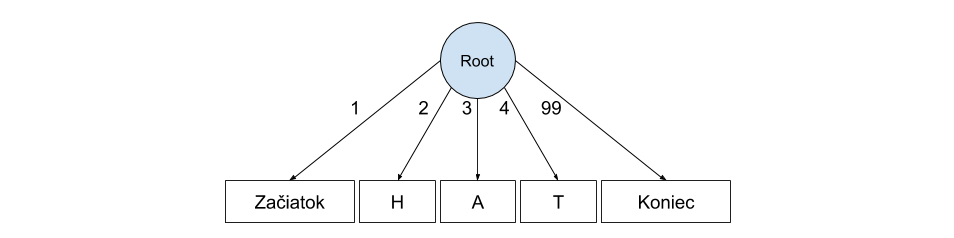
\includegraphics[width=0.6\textwidth]{images/relativne_pozicie1}}
%popis obrazku
\caption[Relatívne pozície znakov]{Relatívne pozície znakov}
%id obrazku, pomocou ktoreho sa budeme na obrazok odvolavat
\label{obr:relativne}
\end{figure}

Pridanie znaku potom funguje veľmi jednoducho. Nájdeme v strome vrcholy medzi ktoré
chceme pridať ďalšie písmeno a ako pozíciu mu dáme priemer relatívnych pozícii daných
vrcholov. Napríklad:
\begin{figure}[H]
\centerline{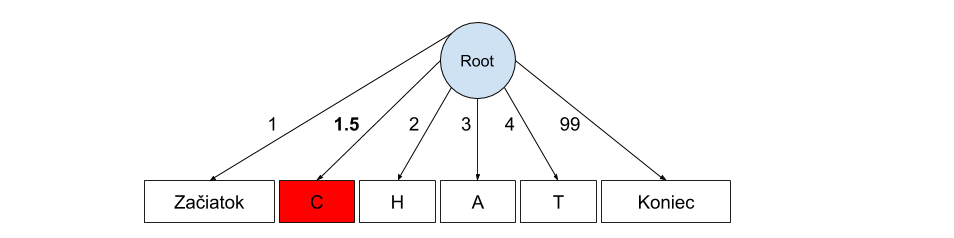
\includegraphics[width=0.6\textwidth]{images/relativne_pozicie2}}
%popis obrazku
\caption[Pridanie relatívnej pozície znakov]{Pridanie relatívnej pozície znakov}
%id obrazku, pomocou ktoreho sa budeme na obrazok odvolavat
\label{obr:relativne_pridanie}
\end{figure}

\begin{flushleft}\textbf {Komutativita a idempotentnosť CRDT}\end{flushleft}
Ak predpokladáme, že pozície spĺňajú podmienky z \ref{def_pozicie}, tak CRDT objekty sú
komutatívne a idempotentné. 

Tým, že všetky relatívne pozície sú unikátne, tak je jedno v akom poradí vykonávame dané operácie,
teda CRDT sú naozaj komutatívne.

Idempotencia je daná tým, že ak chceme do dokumentu pridať znak s najekou relatívnou pozíciou, a tá
sa tam už nachádza, teda znovu pridanie nič neurobí. Ak naopak sa snažíme vymazať niečo na
pozícii, ktorá sa v dokumente už nenachádza, tak vieme, že uz vymazaná bola. Obe operácie teda
zachovávajú idempotentnosť.
\cite{nuno_preguica}

% TODO: obrazky
